\section{Results}
When examining the presence of various game engines on Steam for 2018, 2022, and 2023, it is important to see the significance of these results in the context of indie game development.
The following \autoref{table:steam} presents the percentages of game engines on Steam for these years.

\begin{table}[ht!]
    \resizebox{\columnwidth}{!}{
        \centering
        \begin{tabular}{|l c c c|}
            \hline
            Game Engine & 2018   & 2022    & 2023                                                \\
            \hline\hline
            Unity       & 25.6\% & 61.22\% & $\textcolor{red}{\blacktriangledown 60.04\%}$       \\
            Unreal      & 13.2\% & 15.91\% & $\textcolor{ForestGreen}{\blacktriangleup 16.42\%}$ \\
            Source      & 4.0\%  & 0.27\%  & $\textcolor{red}{\blacktriangledown 0.23\%}$        \\
            CryEngine   & 3.5\%  & 0.23\%  & $\textcolor{red}{\blacktriangledown 0.19\%}$        \\
            GameBryo    & 3.2\%  & -       & -                                                   \\
            IW          & 2.9\%  & -       & -                                                   \\
            Anvil       & 2.5\%  & 0.05\%  & $\textcolor{gray}{\bullet 0.05\%}$                  \\
            id Tech     & 1.7\%  & 0.18\%  & $\textcolor{red}{\blacktriangledown 0.15\%}$        \\
            Essence     & 1.1\%  & -       & -                                                   \\
            Clausewitz  & 1.0\%  & 0.03\%  & $\textcolor{red}{\blacktriangledown 0.02\% }$       \\
            Other       & 48.4\% & 22.17\% & $\textcolor{ForestGreen}{\blacktriangleup 22.94\%}$ \\
            \hline
        \end{tabular}
    }
    \caption{Percentage of total games identified on Steam (data collected 2022-09-30 and 2023-10-21)}
    \label{table:steam}
\end{table}

Game engines that have experienced an increase in their percentage of total games developed in comparison to the previous year(s) are highlighted in green, indicating a positive trend, while those that have seen a decrease are highlighted in red, suggesting a decline in their usage over the same period.
The data from 2018 was collected using the Wikipedia method, while the data from 2022 and 2023 was collected using the pattern matching method.
Color-coding in \autoref{table:steam} is missing for the column for 2022.
This is due to the differing data collection methods used in 2018.
It is difficult to say whether the newer method can attribute more game engines or simply more games were created using a particular game engine.
To illustrate, consider Unity, which has 35.62\% more share of all identified games from 2018 to 2022.
Additionally, it is worth noting that among the game engines analyzed, only the Unreal Engine has consistently exhibited growth over the various years.
This trend holds true when considering both the complete dataset, which includes 2018 data, and the dataset from 2022 and 2023 alone.
The Godot Engine is not listed in \autoref{table:steam} because the paper from Toftedahl and Engström did not include it in their analysis.
Despite this omission, the data remains valuable in shedding light on changing market dynamics. \\

Between 2022 and 2023, it is noteworthy that other game engines have also gained increased popularity, indicating shifts in the competitive landscape.
At the time of the collected data in 2022, 1.15\% of games were created with the Godot Engine.
However, in 2023, this percentage increased to 1.44\%.
Compared to other game engines on SteamDB, the Godot Engine ranks 6th out of 65 recognized game engines.
In addition to that it is important to understand that the percentages from \autoref{table:steam} represent lower bounds.
Particularly in the case of the Godot engine, there could be a lot more games.
This is due to the fact that the Godot Engine allows for the export of executables without a recognizable filename signature, making them unidentifiable by the SteamDB algorithm.
Consequently, only a subset of games with specific filename patterns can be matched. \\

\begin{figure}[ht!]
    \begin{center}
        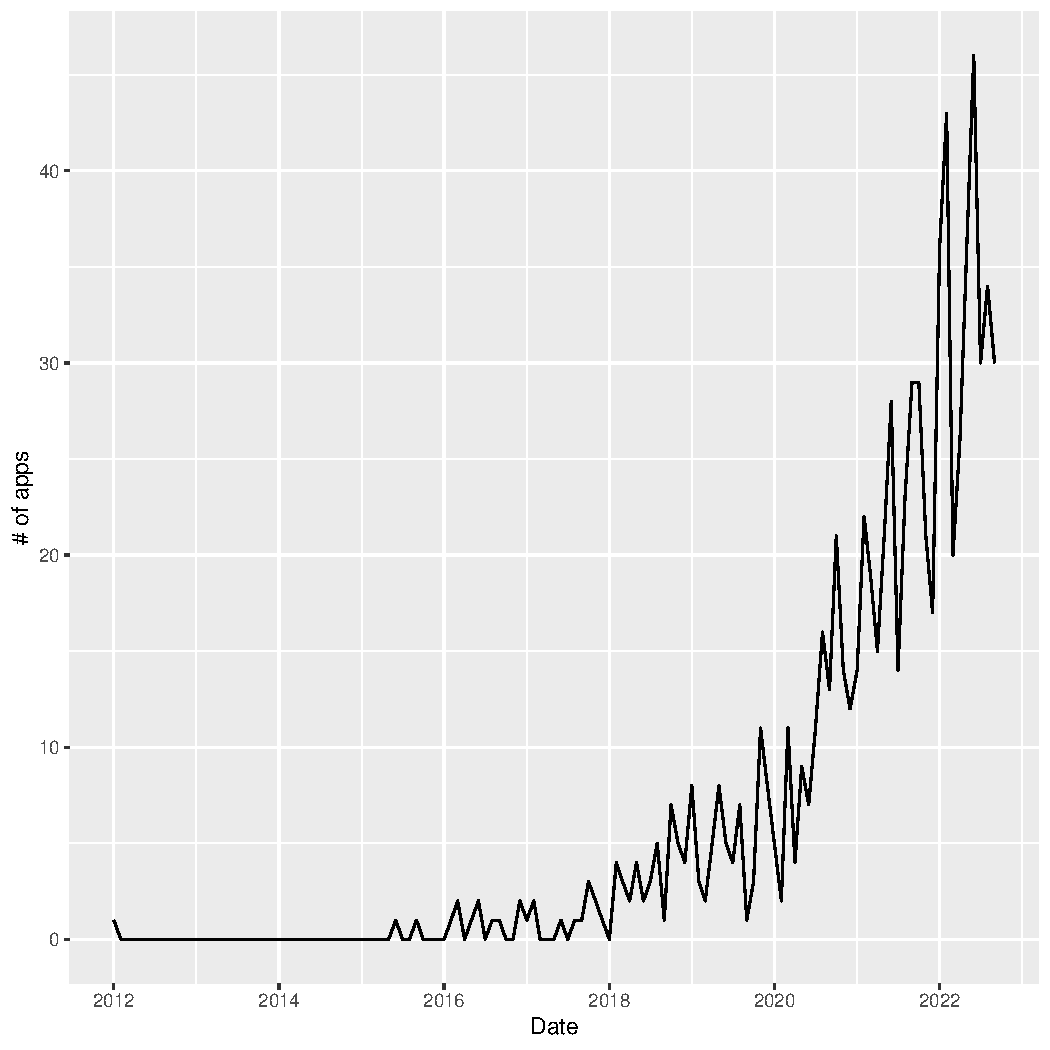
\includegraphics[width=1\columnwidth]{figures/godot-graph.pdf}
        \caption{\label{fig:godot-graph} Number of released Apps on Steam per month}
    \end{center}
\end{figure}

Examining the monthly app releases depicted in \autoref{fig:godot-graph}, a clear trend emerges: in 2020, there was a significant increase in the number of released games.
This increase in game releases prompts further investigation to understand the underlying reasons.
Prior to conducting a more in-depth analysis of the underlying reasons, we first draw a parallel by comparing the data from itch.io.
In contrast to Steam, the digital sales platform itch.io predominantly showcases indie games, aligning with the specific focus of this paper.
Unlike Steam, itch.io possesses an official statistics website that provides information on game engines \cite{itchio-engines}.
However, it's essential to acknowledge that this data might be incomplete due to its reliance on self-reporting.
Therefore, there may be gaps or inaccuracies in the information, a limitation inherent to self-reported data. \\

\begin{table}[ht!]
    \resizebox{\columnwidth}{!}{
        \centering
        \begin{tabular}{|l c c c|}
            \hline
            Game Engine & 2018   & 2022                                                & 2023                                                \\
            \hline\hline
            Unity       & 47.3\% & $\textcolor{ForestGreen}{\blacktriangleup 49.75\%}$ & $\textcolor{red}{\blacktriangledown 46.33\%}$       \\
            Construct   & 12.3\% & $\textcolor{ForestGreen}{\blacktriangleup 13.12\%}$ & $\textcolor{ForestGreen}{\blacktriangleup 13.82\%}$ \\
            GameMaker   & 11.0\% & $\textcolor{red}{\blacktriangledown 7.32\%}$        & $\textcolor{red}{\blacktriangledown 6.95\%}$        \\
            Twine       & 6.2\%  & $\textcolor{red}{\blacktriangledown 5.35\%}$        & $\textcolor{ForestGreen}{\blacktriangleup 6.03\%}$  \\
            RPG Maker   & 3.9\%  & $\textcolor{red}{\blacktriangledown 2.74\%}$        & $\textcolor{ForestGreen}{\blacktriangleup 2.76\%}$  \\
            Bitsy       & 3.3\%  & $\textcolor{red}{\blacktriangledown 3.11\%}$        & $\textcolor{ForestGreen}{\blacktriangleup 3.18\%}$  \\
            PICO-8      & 2.9\%  & $\textcolor{red}{\blacktriangledown 2.68\%}$        & $\textcolor{red}{\blacktriangledown 2.60\%}$        \\
            Unreal      & 2.8\%  & $\textcolor{ForestGreen}{\blacktriangleup 2.92\%}$  & $\textcolor{ForestGreen}{\blacktriangleup 3.01\%}$  \\
            Godot       & 2.5\%  & $\textcolor{ForestGreen}{\blacktriangleup 5.55\%}$  & $\textcolor{ForestGreen}{\blacktriangleup 7.51\%}$  \\
            Ren'Py      & 2.0\%  & $\textcolor{red}{\blacktriangledown 1.93\%}$        & $\textcolor{ForestGreen}{\blacktriangleup 2.07\%}$  \\
            Other       & 5.9\%  & $\textcolor{red}{\blacktriangledown 5.55\%}$        & $\textcolor{ForestGreen}{\blacktriangleup 5.75\%}$  \\
            \hline
        \end{tabular}
    }
    \caption{Percentage of total games identified on itch.io (data collected 2022-09-30 and 2023-10-21)}
    \label{table:itch}
\end{table}

Similar to Steam, the data from itch.io can be compared to the 2018 reference paper using the most current data available from 2022 and 2023.
The consistent data collection method allows for direct comparisons, as illustrated in \autoref{table:itch}.
Upon comparing the data presented in \autoref{table:steam} and \autoref{table:itch}, Unity stands out as a prevalent game engine.
In both 2022 and 2023, Unity consistently constitutes over half of all games on Steam and nearly half on itch.io.
This dominance is particularly striking when considering the second-ranking game engines, which represent approximately 16\% of games on Steam and roughly 14\% on itch.io in 2023.
A similar trend can be observed for 2022. \\

It can also be seen that only three other game engines have consistently gained popularity on itch.io.
These three game engines are Construct, Unreal and the Godot Engine.
Construct is a game engine primarily aimed at non-programmers.
With the help of visual programming, it is intended to make it easier for novice programmers to get started.
The notable increase in its percentage of games may be attributed to the appeal of game development to a broader audience with limited coding expertise.
However, this is only an assumption that needs to be investigated further. \\

Looking at \autoref{table:itch}, it becomes evident that the Godot Engine has experienced remarkable growth in popularity on itch.io.
To delve deeper into this trend, the previously mentioned script was used to compile games from itch.io along with their release dates.
It should be mentioned that not all games could be fetched with this script.
Despite the missing data sets of up to about 10\% of the games, it is still possible to create a trend plot for the game engines listed in \autoref{table:itch}.

\begin{figure}[ht!]
    \begin{center}
        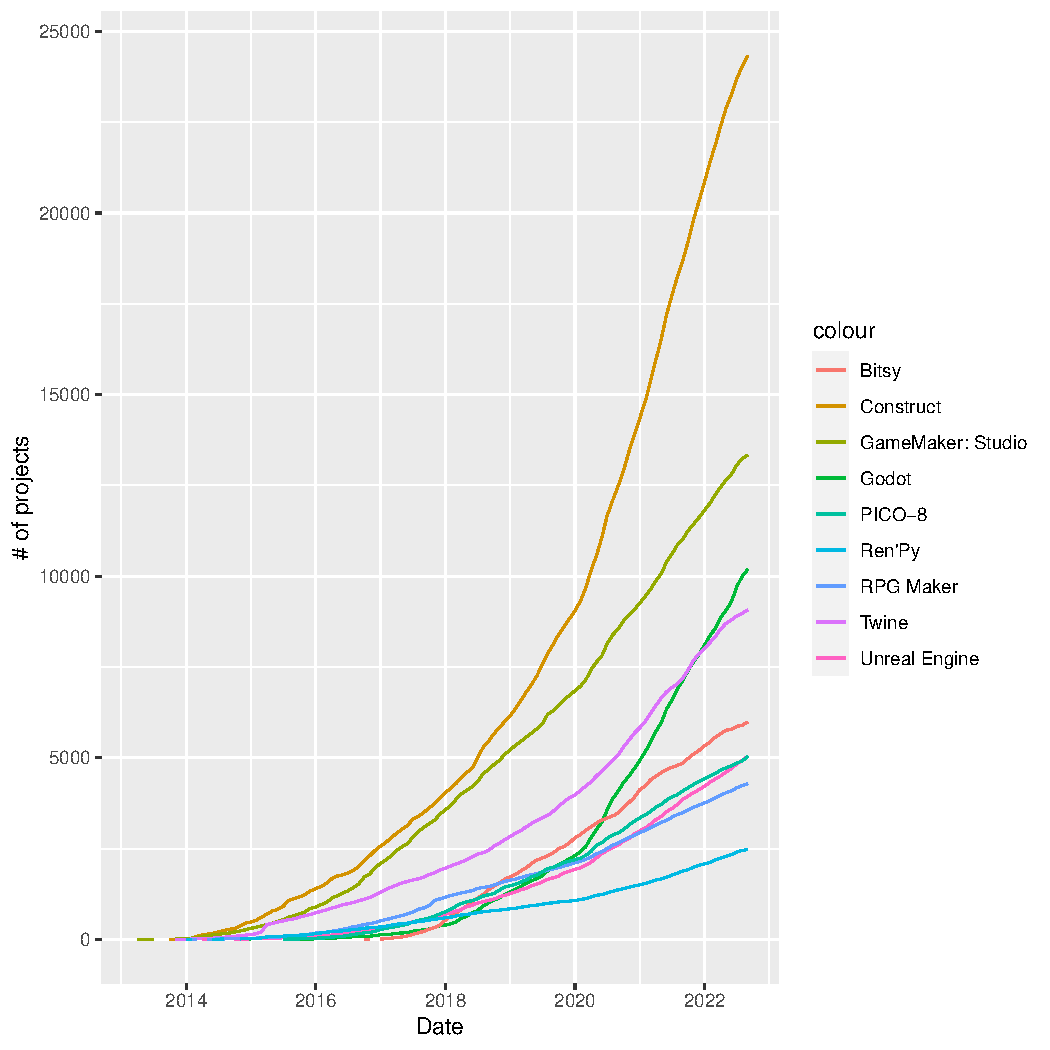
\includegraphics[width=1.1\columnwidth]{figures/trend-graph.pdf}
        \caption{\label{fig:trend-graph} Cumulative sum of the number of projects on itch.io}
    \end{center}
\end{figure}

This graph is shown in \autoref{fig:trend-graph}.
Notably, Unity, due to its large number of projects, has been excluded from the graph to ensure better visibility and clarity for the other game engines.
It is evident that the Godot Engine has gained a significant surge in popularity in 2020, surpassing both Bitsy and Twine.
This analysis has its limitations, as it relies on the quantity of games published.
Quality and quantity of games by individual publishers were not considered.
Determining the exact percentage of indie game studios is challenging as not every publisher was individually analyzed.

\begin{table}[ht!]
    \resizebox{\columnwidth}{!}{
        \centering
        \begin{tabular}{|l c c c c|}
            \hline
            Game Engine & 2020   & 2021                                               & 2022                                               & 2023                                             \\
            \hline\hline
            Unity       & 62.2\% & $\textcolor{red}{\blacktriangledown 61.6\%}$       & $\textcolor{red}{\blacktriangledown 61.1\%}$       & $\textcolor{red}{\blacktriangledown 59\%}$       \\
            Godot       & 12.2\% & $\textcolor{ForestGreen}{\blacktriangleup 13.1\%}$ & $\textcolor{ForestGreen}{\blacktriangleup 15.6\%}$ & $\textcolor{ForestGreen}{\blacktriangleup 19\%}$ \\
            GameMaker   & 10.9\% & $\textcolor{red}{\blacktriangledown 8.9\% }$       & $\textcolor{red}{\blacktriangledown 6.1\%}$        & $\textcolor{red}{\blacktriangledown 5\%}$        \\
            Unreal      & -      & 4.2\%                                              & $\textcolor{ForestGreen}{\blacktriangleup 4.8\%}$  & -                                                \\
            Construct   & 1.7\%  & $\textcolor{ForestGreen}{\blacktriangleup 2.4\%}$  & $\textcolor{red}{\blacktriangledown 1.7\%}$        & -                                                \\
            Stencyl     & 0.1\%  & 0.1\%                                              & -                                                  & -                                                \\
            Other       & 12.9\% & $\textcolor{red}{\blacktriangledown 6.5\%}$        & $\textcolor{ForestGreen}{\blacktriangleup 7.0\%}$  & $\textcolor{ForestGreen}{\blacktriangleup 17\%}$ \\
            No engine   & -      & 3.1\%                                              & $\textcolor{ForestGreen}{\blacktriangleup 3.7\%}$  & -                                                \\
            \hline
        \end{tabular}
    }
    \caption{Used game engines by GMTK Game Jam participants over the years \cite{gmtk-twitter}}
    \label{table:gmtk}
\end{table}

An interesting distinction on itch.io, which is not as prominent on Steam, is the prevalence of games created during game jams, which are defined as follows:
\blockquote{A game jam is an accelerated opportunistic game creation event where a game is created in a relatively short timeframe exploring given design constraint(s) and end results are shared publically \cite{game-jam-definition}.}
With around 18,000 - 23,000 participants and around 6,000 - 7,000 submissions, GMTK Game Jam is the largest past game jam event on itch.io \cite{gmtk-game-jam-2021, gmtk-game-jam-2022, gmtk-game-jam-2023}.
\autoref{table:gmtk} shows the game engines used by participants in the events from 2020 to 2023.
This table is clearly showing that the Godot Engine is the only game engine from the table to outperform the usage of the previous year three years in a row. \\

To explore more about the Godot Engine, the Godot Community Poll from 2022 and 2023 was examined \cite{godot-poll-results-22,godot-poll-results-23}.
In 2022, there were 5,315 responses to the survey, while in 2023 the number increased to 7,671.
These surveys contain answers to a variety of questions.
Regarding previous experiences with other game engines, respondents in the 2022 survey mentioned Unity, other third-party engines, and GameMaker.
In the 2023 survey, the trends remained consistent.
The surveys show that most people heard about the Godot Engine for the first time between 2018 and 2020.
However, most did not start development with the engine until the following years 2019 to 2022.
The surveys also clearly show that the game engine is mainly used for 2D game development.\\

The survey from 2022 sheds light on further facts that are relevant to indie game development.
A substantial 84\% of participants stated that they use the Godot Engine as a hobby, while 9\% identified themselves as full-time indie game developers.
According to the definition outlined in this paper, hobby developers fall under the category of indie game developers, as they share common characteristics such as focusing on specific goals, lacking financial support from larger companies, and working in small teams.
This is further supported by the finding that 97.9\% work on their project alone or in a team of up to five people.
Furthermore, the survey reveals that 83.7\% of respondents do not earn any income from their games, emphasizing their indie status.
Additionally, the two most prevalent digital sales platforms among respondents are itch.io (7.1\%) and Steam (6\%).
